\documentclass[11pt,a4paper,english]{uvamath}
\usepackage[english]{babel}

\usepackage{amsmath, amsfonts, amssymb, a4wide, fancyhdr, lineno, graphicx, epsfig, soul, color, hyperref}
\usepackage[square, numbers]{natbib}

% Running line numbers:
\linenumbers
% Number only every 5:th line:
\modulolinenumbers[5]

%Nodig om een bibliography midden in het artikel te zetten, ipv aan het einde zoals eigenlijk gebruikelijk is
\renewcommand{\bibsection}{}

% TODO command
\newcommand{\todo}[1]{
    \hl{#1}
}

% The things that should be filled in by each group, depending on their situation, are written in a todo command, \todo{like this text}. All text in normal the normal font, is applicable for any group. However, everyone is free to adapt any text, and it is even suggested to look at all text critically and make changes if needed.

% Project specific commands
\author{Tom van Duist \& Kevin van den Bekerom}

\newcommand{\projectname}{\todo{Project Name}\ }


\newcommand{\aanpassen}[1]{ {\sethlcolor{green} \hl{#1}} }

\title{Requirements Document}
%Variables
\newcommand{\TitelAbbr}{RD}
\newcommand{\Version}{0.1}
\newcommand{\rreport}{Intermediate Requirements Engineering report}



\what{Lab assignment Requirements Engineering}
\supervisors{}
\author{Tom van Duist \& Kevin van den Bekerom}



\begin{document}

\maketitle


\tableofcontents

\chapter*{Document Status Sheet}
\section*{Document status overview}
\subsection*{General}
\begin{tabular}[!]{ll}
    Document title:     & Architectural Design Document\\
    Authors:           	& Kevin van den Bekerom \\ 
						& Tom van Duist \\
    Document status:    & Draft release\\
\end{tabular}

\subsection*{Document history}
\begin{tabular}[!]{|l|l|l|l|}
    \hline
    \emph{Version}    &   \emph{Date} &  \emph{Reason of change}\\
    \hline
    0.0 & 02-09-2015 &  Setup of the document layout\\    
    \hline
    0.1 & 29-10-2015 & Release version week 1 \\
    \hline
\end{tabular}

\clearpage

%\section*{Document Change Records since previous issue}
%\subsection*{General}
%\begin{tabular}[!]{ll}
%   Datum:          &   2015-06-09 \\
%    Document title: &   Architectural Design Document (ADD)\\
%    Identification:  &   \TitelAbbr\_\Version.pdf\\
%\end{tabular}

%\subsection*{Changes}
%\begin{tabular}[!]{|l|l|p{8 cm}|}
%    \hline
%    \emph{Chapter} &   \emph{Paragraph}    &   \emph{Reason to change}\\
%    \hline
%    \ref{c:main_fun} &  whole chapter      & Make prioritizing clear using Moscov model. Clarified functionalities. \\
%    \hline
%    dfdf& tt & ff. \\
%    \hline
%\end{tabular} 

%\chapter{Introduction}
%Blabla.
\chapter{Introduction}
This RD is comprised of knowledge gathered in 4 weeks of Requirements Engineering for the Requirements Engineering class as part of the master education Software Engineering. We have condensed the acquired knowledge of four weeks into one document following the structure of our project plan, see Chapter \ref{pp}. We revised this project plan based on feedback in the second week session with Hans. In the elicitation phase we conducted numerous interviews, which are accessible on our portfolio website, see \todo{website adres}.

\chapter{Project Plan}
\label{pp}
The project plan for the first four weeks is explained in this chapter. The goal is to discover some of the essential features that should be provided by the successor of Blackboard. We base our project plan on the requirements engineering process, see Figure \ref{fig:spiral_model} \cite{RE_book} (chapter 1.1.6). This book identifies four phases of requirements engineering; 

\begin{enumerate}
	\item Domain understanding and elicitation.
	\item Evaluation and negotiation.
	\item Specification and documentation.
	\item Quality assurance.
\end{enumerate}

During the first week we will get familiar with the problem world, as described in the first phase \cite{RE_book}. We will investigate the system-as-is, ourselves, and ask users (students) about their experiences. We will work trough the questions listed in the relevant section in the book. We will also compose a list of stakeholders, which we interview in the coming weeks.

Week 2 will resolve around the second phase: evaluation and negotiation. The goal of this week is to find all critical (business) goals of the stakeholders of the system. Why is it replaced? What is the relation to the mission and vision of the UvA (if there is any)? Why did the UvA use an education management tool in the first place? What are the goals of the students in relation to the tool etc. During this week we will interview remaining stakeholders, to verify and add upon the information we gathered in the first week. We will also interview more students with prepared questions.

%During week 3 we will draft an initial set of requirements. After week 3 the first draft version of the Requirements Document is finished. We will focus on the smallest set of requirements that together realize the business goals on an acceptable level, due to limited time. 

%In week 4 we will plan meetings with relevant stakeholders to asses the set of requirements we drafted for the new system. Assessment focuses on whether we forgot crucial requirements and if the requirements are consistent.  

In week 3 and 4 we will try to answer the questions we deemed most interesting and essential to get a good successor of Blackboard. These can be found in Chapter \ref{ch:elicitation}.

Note that we conduct one round of the spiral model, see Figure \ref{fig:spiral_model}. There will be some backtracking to other phases (previous weeks), because some information becomes available after the relevant week/phase. 

\begin{figure}[h]
	\centering
	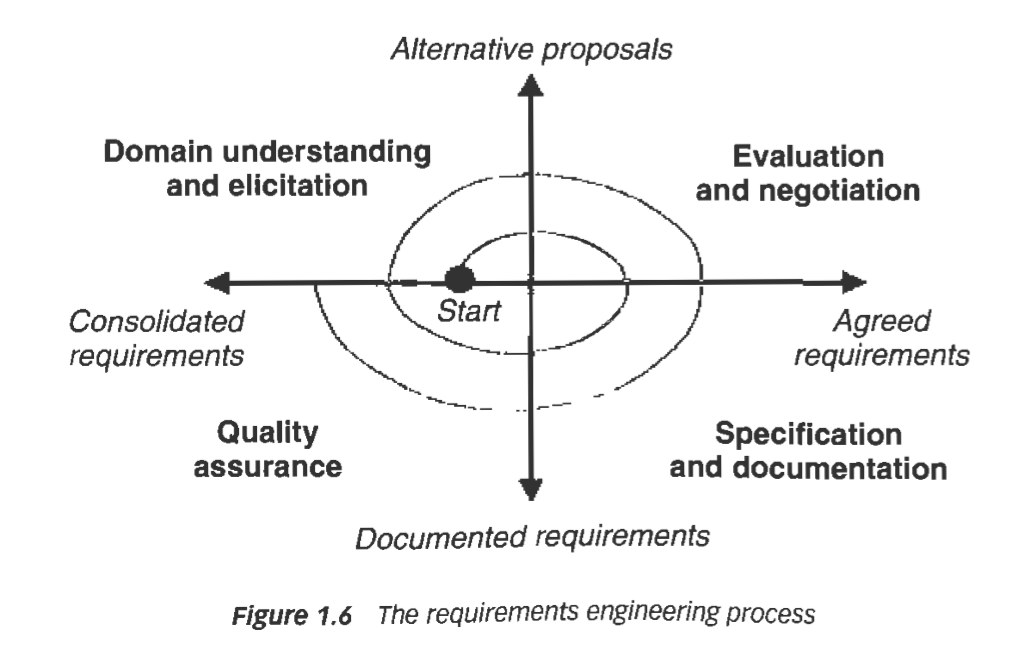
\includegraphics[width=0.75\linewidth]{images/re_process}
	\caption{Spiral Model of requirements engineering process}
	\label{fig:spiral_model}
\end{figure}


\chapter{Domain Understanding}
In the first week we focused on getting a better understanding of the domain in order to form a better understanding of the problems in the domain with relation to the goals, which we will gather during the next phase.

\section{Glossary of terms}
\begin{itemize}
	\item[\textbf{student}] A person who studies at an university (in our case the University of Amsterdam).
	\item[\textbf{teacher}] A person who teachers courses at an university (in our case the University of Amsterdam).
	\item[\textbf{UvA}] University of Amsterdam. 
	\item[\textbf{Blackboard}] Name of currently licensed ELE by the UvA. 
	\item[\textbf{ELE}] Electronic Learning Environment. ICT solution where part of a course teaching and organization is moved to an (online) software platform. An example of an ELE is Blackboard.
	\item[\textbf{ICT}] Information and Communication Technology. Mainly a Dutch term for \textbf{IT}, which stands for Information Technology.
	
\end{itemize}

\section{Organization}
The organization in which Blackboard is used is the University of Amsterdam (UvA). The UvA employs many different IT systems, some of them communicating with Blackboard. The mission and (business) goals of the UvA can be found in Section \ref{uva_goals}. The ICT-department within the UvA has as responsibility to keep all the IT solutions up and running. Teachers using Blackboard have to request new functionality (in practice a request for a new module for Blackboard) at the ICT-department. 


\section{Goal}
The goal of a requirement engineering project in a perfect world would be strife to find all of most important quality requirements for all relevant stakeholders. As stated in Contextual Design \cite{contextual_design} a design process could always be further elaborated, so finding all and every requirements for all stakeholders is an illusion.

Because of this and the time constraints of this project, the goal will be limited to the following: \emph{find a couple of the major requirements for the main stakeholder(s) by asking the right questions}. We believe this is measurable enough for the assignment given the time frame but still enough of an abstraction given that we do not yet have a clear enough understanding of the domain at this time to make it more concrete without taking away from the achieveability.

\section{Scope}
We looked at the functionality of Blackboard. Different IT systems within the UvA that have some connection with Blackboard are not the focus of this study. Aggregated functionality of Blackboard includes:
\begin{enumerate}
	\item Form groups, assign to groups.
	\item Announcements
	\item Share course related files (lectures, papers, assignments, etc).
	\item Grades
	\item Formative tests
	\item Online cooperation
	\item (A)synchronous meetings
	\item Guided self-study
\end{enumerate}


\section{Stakeholders}
\begin{itemize}
	\item Users: Both students and teachers
	\item Management UvA
	\item Blackboard (company)
	\item ICT-department
\end{itemize}

\section{Stakeholder goals}\label{ch:stakeholder_goals}
\subsection{UvA}
\label{uva_goals}
Taken from the core values of the UvA is the following: \\
\textit{Engagement for the UvA and its staff implies the age-old obligation – based on a privileged academic position – to use acquired knowledge and insights to play an ongoing, prominent and visible role in the social debate. This value also reveals that the UvA is committed to the maximum development of the individual talents of its staff and students. Additionally, the choice of this core value suggests a strong mutual involvement between students, staff, employees, study programmes, institutes and the institution as a whole. And, lastly, there is an important link between academia and society. The UvA is located in historical and modern buildings throughout the city of Amsterdam, thus making it an integral part of the city.}

Important goals are:
\begin{enumerate}
	\item The UvA is committed to the maximum development of the individual talents of its staff and students.\cite{uva_mission}
	\item The UvA strives for a strong mutual involvement between students, staff, employees, study programs, institutes and the institution as a whole.\cite{uva_mission}
	\item Evidenced-based ICT innovations are incorporated into the UvA’s education policy.\cite{uva_strategic_plan} \begin{enumerate}
		\item (Strategy): The use of Open Educational Resources – as part of blended curricula – will be one of the educational innovations implemented. ICT policy will be tailored in part to support the education process. 
	\end{enumerate}
	\item A modular Lifelong Learning programme is developed.\cite{uva_strategic_plan} \begin{enumerate}
		\item (Strategy): This programme will draw on the online
		courses in our blended curricula. 
	\end{enumerate}
\end{enumerate}

\subsection{Teacher}
Taken from the UvA goal and by talking to teachers.
\begin{enumerate}
	\item Develop individual skills.
	\item Convey knowledge to students.
\end{enumerate}

\subsection{student}
The student goals still need to be confirmed by finding a relevant paper. As a result of our elicitations we believe these are the broad goals of students.
\begin{enumerate}
	\item Optimally develop one's personal and academic skills.	
	\item Obtain diploma.
\end{enumerate}

\section{Strengths and Weaknesses}
Students: (Based on 3 weeks of interviewing)
\begin{itemize}
	\item[+] Possible to get mobile notifications through the app.
    \item[+] Central point of information access.
	\item[+] Latest schedule of a course.
	\item[-] Hard to use in the beginning.
	\item[-] Different structure per course.
  i.e. "We \textit{have} to use it."
	\item[-] Ugly.
\end{itemize}

We gathered no, or not enough, information about the other stakeholders to draw reliable conclusions about their perceived strengths and weaknesses of the system-as-is.


\section{Domain facts}
\begin{enumerate}                                                           
	\item Formative feedback can help students improve their work.\cite{ict_study} \textit{BB does not offer formative feedback, this is merely a responsibility of the teacher.}
	\item Should be clear link between learning goals (of a course) and the ICT solution. If the ICT solution is merely a means to reach a goal it will not improve learning. \cite{ict_study}\todo{Blackboard is a means to achieve an end. e.g. need information to pass course. Info aonly on BB. Need to hand in assignments. Sometimes only on BB.  Verwerken als antwoord op een van onze vragen. Ref naar deze domain rule. Students gebruiken BB alleen als teacher dit ook gebruikt.}
	\item Important how ICT is used that determines its effectiveness.\cite{ict_study} \todo{If a domain fact is that students use BB because they have to, then a BB-related solution might not be effective. Combine this domain fact with answer to the question. Richard zijn doc zegt dit eigenlijk ook. STudents gebruiken omdat teachers verplicht stellen.}
	\item Teachers use ICT based on their own skills. This might undermine its effectiveness.\cite{ict_study} \todo{Data van Richard gebruiken!! e.g. 20 procent intrinsically motivated teachers, 80 procent doet maar wat.}
	\item ICT changes rapidly. (Moore's Law)
	\item The availability of a tool does not determine its effectiveness. In its initial stages the focus is on how to use the tool, rather than using the tool for learning-promoting purposes. \cite{ict_study}
	\item Research also rarely reports on technical issues or problems with equipment, yet these are what teachers find act as barriers to increasing the use of technology in classrooms.\cite{ict_study} \todo{Take away barrier by stripping non-essential functionality??}
	\item Media reports faster on trends then research can validate or discredit using that technology.\cite{ict_study} Example: \todo{Interactive Whiteboards}. 
	\item ICT does not help increase pupils attainment.\cite{ict_study}
	\item (Digital) instant feedback significantly improves student learning \cite{clicker}
	\item Advanced Blackboard functionality is almost never used. Adaptive rules 5.9$\%$ in 2014/2015. Progress warnings $< 1 \%$. \cite{richard_report}
\end{enumerate}


\chapter{Elicitation phase}\label{ch:elicitation}
During this phase we will try and answer some important domain questions (though we may not be able to answer them all) and update the information once we get new data.

\section{What are the essential features of the Blackboard (or similar ELE) system for the users?}
In order to find the essential features of the Blackboard system we have performed elicitations amongst both teachers and students. From these we have devised the following preliminary list of essential features:

\begin{itemize}
	\item Teacher:
	\begin{itemize}
		\item Publishing documents
		\item Publishing assignments
		\item Publishing announcements
	\end{itemize}
	
	\item Student:
	\begin{itemize}
		\item Retrieve relevant information/documents.
		\item Hand in digital assignments.
	\end{itemize}
\end{itemize}

We can distil this into a single feature list:
\begin{itemize}
	\item Share documents.
	\item Hand in digital assignments.
	\item Publish announcements.
\end{itemize}
We wanted to quantify this data with the actual use as logged by the ICT department of the UvA, but our request for information has been rejected.

\section{To what extend does the current Blackboard system support the UvA goals?} \label{uva_goal_question}
In order to answer this question we have divided it into two sub-questions. As the main goal of the UvA (see \ref{ch:stakeholder_goals}: \nameref{ch:stakeholder_goals}) could be divided into sub-goals for its staff and students we have done the same with this question to make it easier to answer.

\subsection{To what extends does the system support the goals of the teachers?}
By reasoning about how teachers develop their skills, from personal experience by looking around in the UvA and talking to teachers we can answer this question for the staff:
\begin{itemize}
	\item Teachers do not develop their skills through Blackboard, they develoop their skills by performing activities related to their field. For example by developing assignments for students. Or by doing personal research, read papers, go to conferences etc.
\end{itemize}

\subsection{To what extends does the system support the goals of the students?}
By talking to teachers we have answered this question for students:
\begin{itemize}
	\item Students do not develop their skills through Blackboard because the system does not create \emph{good} teachers. Students develop their skills through individual discipline and programs set up by competent teachers, Blackboard is just one of the many tools used by the teachers. It still boils down to the teacher himself to channel his knowledge.
\end{itemize}

\section{Which type of usability problems have no impact on education?}\label{s_1}
\subsection{What usability issues arise from using Blackboard?}
From our elicitations with and talking to students we learned Blackboard has the following usability issues:
\begin{itemize}
	\item Many clicks to reach the target destination.
	\item Convoluted User Interface.
	\item No generic structure for storing documents. Every teacher uses his own file structure.
	\item Tiny buttons.
	\item Non-intuitive user interface. Blackboard was difficult to use in the early stages ($<$2 months).
	\item Ugly, outdated design.
\end{itemize}
When asked how these usability issues affected the learning process of the students, every students said it didn't affect their learning process, but was merely an annoyance. For certain issues (No generic structure, tiny buttons, non-intuitive interface) they learned to adapt.

\section{What characteristics of users are important to consider for the selection of a new system?}
To answer this question we first set out to find different characteristics of users through our elicitations, focusing mainly on their study goals and use of resources to this end. What we encountered was not really what we expected. Obviously all students want to pass their exams and eventually earn a degree, but besides this most students want to develop specific skills, broaden or deepen their knowledge base; earn intrinsic knowledge to some degree. What we found was:
\begin{itemize}
	\item Irrespective of the degree of intrinsic knowledge the student seeks, he uses other sources of information than those solely provided by their teacher (be it through Blackboard or other means).
\end{itemize}
So we found that irrespective of the characteristics regarding study goals of the student, he independently uses resources outside of the ELE to get additional information to help achieve these goals.

\section{What factors in education improve student learning?}
\subsection{Does the usage of Blackboard save the teachers time as compared to organizing the course themselves (file sharing, group building, assignment checking for plagiarism, etc)?}
\label{ss_1}
\subsection{Will teachers who spent (relatively) less time on bureaucracy improve student learning, i.e. perform activities in the \textit{education improvement factors} set?}
\label{ss_2}

\section{opportunities arising from technology}
During the interviews we found out that students use communication channels not integrated into Blackboard. Named examples are Facebook, Slack and Whatsapp. These IT solutions were used to discuss answers to assignments, among others. If we were to implement these into the new ELE, we have to investigate their concrete effect on student goals, as stated in \ref{ch:stakeholder_goals}: \nameref{ch:stakeholder_goals}.

The \rreport showed that teachers only use the basic functionality of Blackboard. We identified what basic functionality entails, which can be read in \todo{Reference to essential functionality section}. The interviews showed that all students knew about, and used the essential functionalities. As already noted, students only use Blackboard, when their teacher uses Blackboard. We can hypothesize that if a teacher does not use the more advanced functionality (i.e. message boards), student wont either. Our interview data is not extensive enough to confirm or disprove this hypothesis. We also did not ask the right questions. 

   \todo{Also privacy! Integration with other IT systems within the UvA, i.e. information integrity. (Organiztional and techical constraints)}
\section{Organizational and technical constraints}
The UvA consists of many different departments (Amsterdam University College, Department of Medicine, Department of Law, Department of Sciences among others). In the \rreport it is stated that there are significant differences in the usage of Blackboard among different departments. The diversity of education is one thing to take into account. Raquel Benbunan-Fich \cite{improveEducationWithIt} identified two models of content transmission: the objectivist and constructivism model. The first is classified by the typical classroom example, where a teacher conveys knowledge to students as a one-way stream of information. For the latter, knowledge emerges through peer interaction, evaluation and cooperation. For each model there are different IT solutions. The first model relies more on sharing content, the second on communication channels (such as Slack). As mentioned before, students already make extensive use of communication channels without Blackboard. \\
\todo{The domain properties that are necessary for
	the software-to-be to work properly.} 

For the new ELE we will assume that students who have to use the system to pass their courses, will use the system, even if the new ELE has usability issues. These usability issues can be of the same order of magnitude as the usability issues Blackboard has. See \todo{Ref to usability issues} for a list of issues we found. 

\section{Summary of important findings}
\begin{itemize}
	\item The essential features of Blackboard are:
	\begin{itemize}
		\item Share documents.
		\item Hand in digital assignments.
		\item Publish announcements.
	\end{itemize}
	\item Blackboard does not intrinsically support the goals of the teachers and students.
	\item All types of students use different sources in addition to Blackboard to get information.
	\item Some usability issues do not affect the learning process of the students.
\end{itemize}


\chapter{Evaluation and Agreement}
In this chapter we will evaluate and negotiate our findings. On conflicting concerns an agreement must be met which will be grounded in data gathered in the previous phases.
\todo{Italic text is a begin on how to answer these questions. Work out what is relevant using the information we obtained in Chapter 4.}
\section{Does the new Blackboard have to contribute to the goals of the UvA?}
As we found out when answering "\emph{\ref{uva_goal_question}: \nameref{uva_goal_question}}", we doubt if the current system has a notable contribution towards the main goal of the UvA and are not sure if such a system ever will, although this is hard to answer.

A different UvA objective states: \emph{Evidenced-based ICT innovations are	incorporated into the UvA’s education policy} \cite{uva_strategic_plan}.

Tailoring the requirements of the new system to fit this objective might be an easier task to accomplish. Is this a good goal however? We think it isn't. It cannot be refuted - Evidenced-based ICT innovation showing what? - , therefore the goal is ambiguous. Our solution, whatever form it might take, can be easily transformed to satisfy an ambiguous goal by the nature of ambiguously. We can just interpret the goal in favour of our solution. 

\section{Necessary features}
As we saw in \emph{\ref{ch:elicitation}: \nameref{ch:elicitation}} the necessary features according to almost all of the users are \emph{sharing documents}, \emph{Hand in assignments} and \emph{Publish announcements}. According to Richard van der Wurff's research only a small subset of teachers use the other functionalities of Blackboard. Also these teachers are the innovative users that use different tools next to Blackboard \cite{richard_report}. 

According to these findings we believe that a system where the core functionalities that all users use is supported, and all other tool use falls outside of this system would suffice for the stakeholder needs that we identified. Thus a system that supports the bare minimum of features would suffice.

\begin{itemize}
	\item Conflicting concerns must be identified and resolved. These often arise from multiple
	viewpoints and different expectations. For instance \textit{Usability vs Goal of students OR goals of UvA vs goals of students.}
	\item There are risks associated with the system that is being shaped. They must be assessed
	and resolved. {Privacy, accessibility of tools, and their reliability.}
	\item \textbf{The alternative options} identified during elicitation must be selected on that basis. \todo{Do we have alternative options?}
	\item Requirements prioritization is often necessary for a number of reasons: 
	\begin{itemize}
		\item Favouring higher-priority requirements is a standard way of resolving conflicts.
		\item Dropping lower-priority requirements provides a way of integrating multiple wishlists
		that would together exceed budgets and deadlines.
		\item Priorities make it easier to plan an incremental development process, and to replan
		the project during development as new constraints arise such as unanticipated delays,
		budget restrictions, deadline contractions etc.
	\end{itemize}
\end{itemize}

\chapter{Specification and Documentation}
This section concludes our Requirements Document by listing the requirements that we found, next we state our vision for the successor of Blackboard according to these requirements and finally we argue why our findings are reliable or not reliable.

\section{Requirements}
According tot he goals that the new system must adhere to we have created \emph{goal contribution trees} \cite{RE_book}. We have subdivided each goal into sub-goals until each goal only affected one agent, these are the requirements. Thus the leafs of each tree is a requirement for his parent goal (unless stated otherwise).
\subsection{Requirement: Share documents}
\begin{figure}[h!]
	\centering
	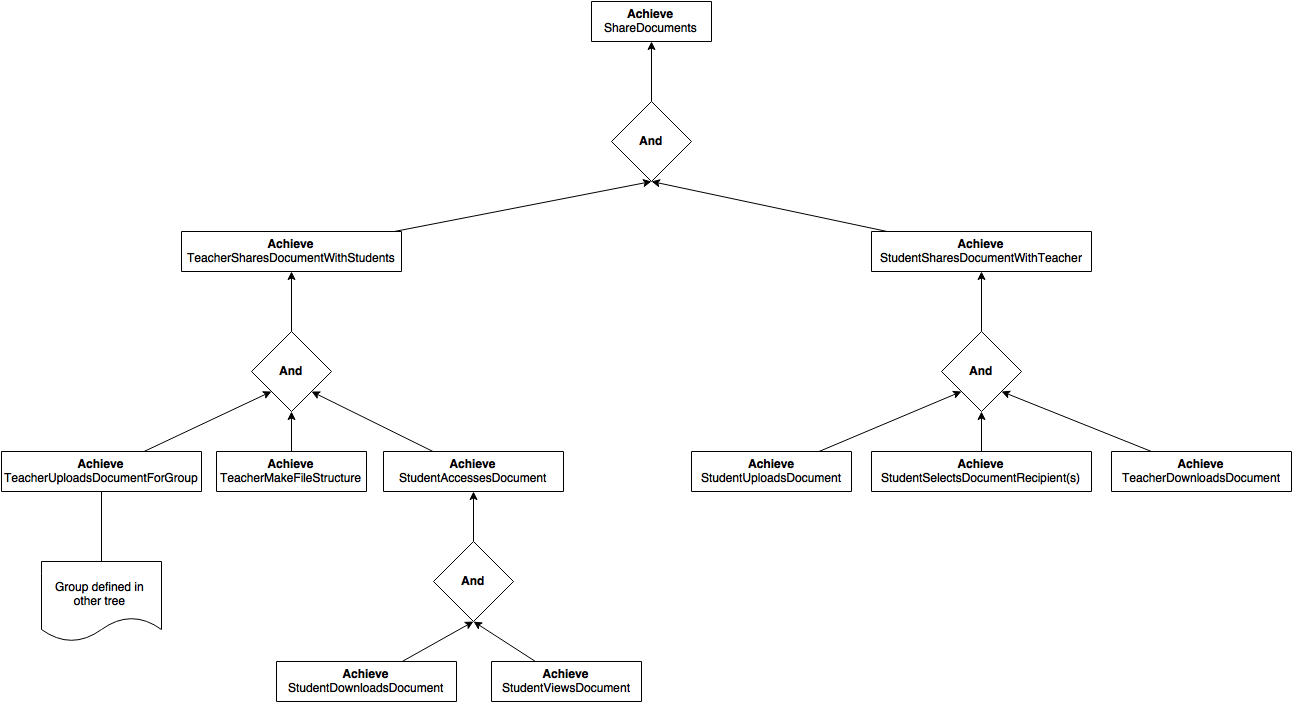
\includegraphics[width=1\linewidth]{images/ShareDocuments.png}
	\caption{Share documents goal contributions.}
	\label{fig:goal_share_documents}
\end{figure}

\clearpage
\subsection{Requirement: Hand in assignments}
\begin{figure}[h!]
	\centering
	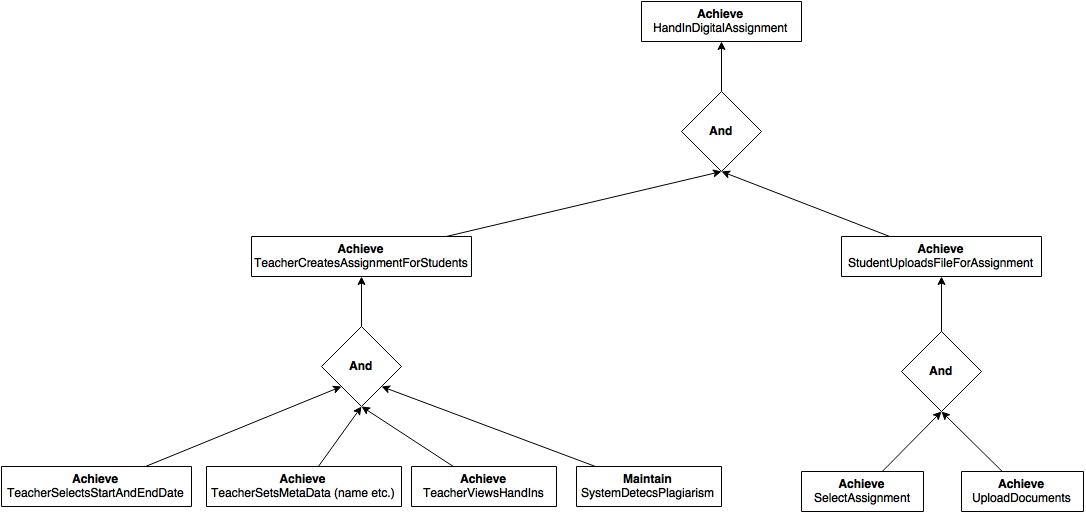
\includegraphics[width=1\linewidth]{images/HandInAssignment.png}
	\caption{Hand in assignments goal contributions.}
	\label{fig:goal_hand_in_assignments}
\end{figure}

\clearpage
\subsection{Requirement: Publish announcements}
\begin{figure}[h!]
	\centering
	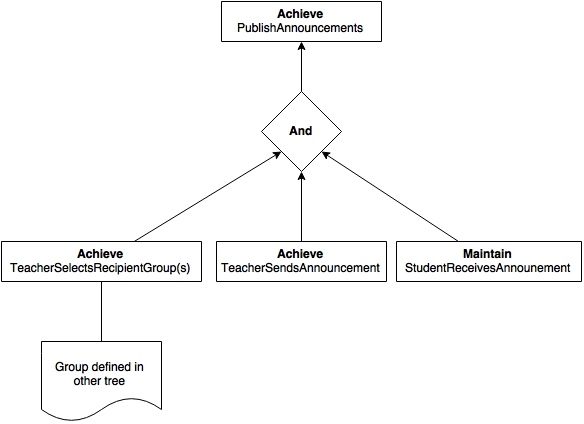
\includegraphics[width=1\linewidth]{images/PublishAnnouncements.png}
	\caption{Publish announcements goal contributions.}
	\label{fig:goal_publish_announcements}
\end{figure}

\clearpage
\subsection{Requirement: Manage student groups}
\begin{figure}[h!]
	\centering
	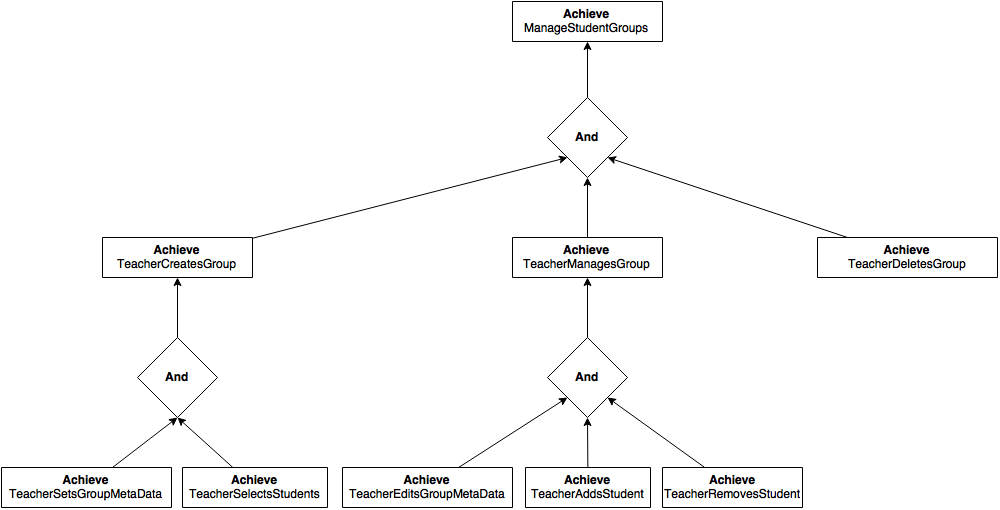
\includegraphics[width=1\linewidth]{images/ManageStudentGroups.png}
	\caption{Manage student groups goal contributions.}
	\label{fig:goal_manage_student_groups}
\end{figure}

\section{Vision}
According to our findings as laid out in this document we believe that the current Blackboard already offers too much functionality. As we saw in \emph{\ref{ch:elicitation}: \nameref{ch:elicitation}}

\clearpage
\section{Reliability}
The sources of most of our information are the elicitations (unless stated otherwise) that we performed, but also our own experience, and talking to the users (students and teachers).

Because our sample size for these answers is really low compared to the number of users of the system. And both teachers and ourself are just talking about personal experiences and beliefs many of the presented facts that have the elicitations as source are not very reliable. We would be able.
Also as we later learned from reading Thinking, Fast and Slow by Kahneman, people are not eager to open up and possibly embarrass themselves. So they might not let us know that they, for example, find Blackboard hard to use. As it might show that they personally do not have the skills to use the tool, which they can experience as embarrassing.

To get more reliable answers we could substitute the questions regarding usability by different questions, which are not directed personally at the interviewee, but are harder for him to answer. As Kahneman showed, in his mind the interviewee will (unconsciously) substitute the question by looking at his own experience (and of people around him), which is the answer that we are looking for.

In conclusion our findings are not very reliable because:
\begin{itemize}
	\item Small sample size
	\item Only interviewed within one domain (again sample size)
	\item Biased interviewer
	\item Received abstract answers
	\item Based some data on own experience, and that of fellow students
\end{itemize}
We only learned later in the course how to avoid above examples. If we would have the time and resources to properly interview enough people, and quantify the data with proper research this would strengthen the reliability of the conclusion.










\chapter{Negotiation}
As we found in \emph{\ref{ch:understanding} \nameref{ch:understanding}} a system like Blackboard does not support the UvA goals, it is merely a tool that staff and students use to achieve their goals. Moreover the UvA objectives that relate to the use of ICT are defined in such an ambiguous way that any system could satisfy them with little effort.

Because of this we will focus only on the essential features of the ELE, the (un)usability of the system and the minimum system that will support this. Because of the workable usability problems that we found (see \ref{s_1}) we believe that a system which integrates all the essential features in a single system is not required. It can be a plus but it is not a requirement if other requirements such as cost (which we did not research) ar deemed more important.


\chapter{Requirements}
In this chapter we will start by forming high level goals the new system has to meet. These are distilled from our domain knowledge and understanding, combined with the goals of the different stakeholders. Unreachable goals are filtered out. From these goals we will recursively state subgoals until we reach goals satisfying a single actor (stakeholder). We call this a leaf of the goal-tree. All leaves of the goal-tree are requirements for the new system, according to Van Lamsweerde \cite{RE_book}.

\chapter{Recommendations}
\todo{refactor into different chapter}
The following questions where not investigated due to time constrainst. However, we believe these questions are very important due to reasons explained below. We provide suggestions on how to obtain the answers to these questions, such that the \textit{Werkgroep Toekomst Elektronische Leeromgeving} can implement our methods and obtain the correct information, i.e. relevant to stakeholder and business goals.

\section{Does Blackboard improve learning?}
The question can be made concrete by asking:\textbf{ What is the relation between Blackboard usage (in percentage) and student's grades?} \textit{Werkgroep Toekomst Elektronische Leeromgeving} already has the Blackboard usage data. They simply need to combine this data with student grades (link course average grades to course Blackboard usage). \\

In fact, by linking average course grades to usage, we can even answer other important questions:
\begin{enumerate}
	\item Does usage of advanced Blackboard functionality (e.g. Adaptive Rules) warrant an increase in education quality, measured by student grades? We can hypothesize that is does warrant an increase in education quality, and try to reject the null hypothesis.
	\item Are there big differences between courses (average grades) when Blackboard usage is about the same, but the courses differ in being more constructive (focussed on peer interaction) or objective (classical lecture room idiom, teacher conveys knowledge as one-way stream of information), see \cite{improveEducationWithIt}. 
\end{enumerate}

Important to note is that we need to take into account the difficulty of each different course. We cannot simply compare the average grades of two courses since they will differ in difficulty. A remedy for this is look for courses that have an increase or decrease in Blackboard usage over the years. 


\chapter{References}

\begin{thebibliography}{9}
	
	\bibitem{contextual_design}
	Hugh Beyerand and Karen Holtzblatt,
	\emph{Contextual Design},
	
	\bibitem{RE_book}
	Axel van Lamsweerde,
	\emph{Requirements Engineering: From System Goals to UML Models to Software Specifications}
	
	\bibitem{ict_study}
	Steve Higgins,
	\emph{Does ICT improve learning and teaching in schools},
	Newcastle University.
	
	\bibitem{uva_mission}
	UvA mission \\
	\url{https://www.uva.nl/en/about-the-uva/uva-profile/mission-and-identity/core-values-and-ambitions/core-values-and-ambitions.html}
	
	\bibitem{uva_strategic_plan}
	University of Amsterdam,
	Strategic Plan 2015-2020 - Boundless Curiosity \\
	\url{https://www.uva.nl/binaries/content/assets/uva/en/about-the-uva/uva-profile/mission-and-identity/boundless-curiosity-2015-2020-nieuw-en.pdf?2870291918297}
	
	\bibitem{improveEducationWithIt}
	Raquel Benbunan-Fich,
	\emph{Improving Education and Training With IT},
	COMMUNICATIONS OF THE ACM June 2002/Vol. 45, No. 6
	
	\bibitem{clicker}
	Steven A. Yourstone,† Howard S. Kraye, and Gerald Albaum,
	\emph{Classroom Questioning with Immediate Electronic Response: Do Clickers Improve Learning?},
	Decision Sciences Journal of Innovative Education Volume 6 Number 1,
	January 2008
	
	\bibitem{richard_report}
	Werkgroep Toekomst Elektronische Leeromgeving,
	\emph{Tussenrapport Versie 2.3 28 oktober 2015}
	

	
\end{thebibliography}


\appendix


\end{document}
